This manuscript
(\href{https://SORTEE-Github-Hackathon.github.io/manuscript/v/956112ff108905503babe0eed04fa5ef9ddcd12b/}{permalink})
was automatically generated
from \href{https://github.com/SORTEE-Github-Hackathon/manuscript/tree/956112ff108905503babe0eed04fa5ef9ddcd12b}{SORTEE-Github-Hackathon/manuscript@956112f}
on July 14, 2022.

\hypertarget{authors}{%
\subsection{Authors}\label{authors}}

\begin{itemize}
\item
  \textbf{Robert Crystal-Ornelas}
  \includegraphics[width=0.16667in,height=0.16667in]{images/orcid.svg}
  \href{https://orcid.org/0000-0002-6339-1139}{0000-0002-6339-1139}
  · 
\includegraphics[width=0.16667in,height=0.16667in]{images/github.svg}
  \href{https://github.com/robcrystalornelas}{robcrystalornelas}
  · \includegraphics[width=0.16667in,height=0.16667in]{images/twitter.svg}
  \href{https://twitter.com/rob_c_ornelas}{rob\_c\_ornelas}
  Earth and Environmental Sciences Area, Lawrence Berkeley National Laboratory, Berkeley, CA 94720, USA
\item
  \textbf{Brandon P.M. Edwards}
  \includegraphics[width=0.16667in,height=0.16667in]{images/orcid.svg}
  \href{https://orcid.org/0000-0003-0865-3076}{0000-0003-0865-3076}
  · 
\includegraphics[width=0.16667in,height=0.16667in]{images/github.svg}
  \href{https://github.com/BrandonEdwards}{BrandonEdwards}
  Department of Biology, Carleton University, Ottawa, ON K1S 5B6, Canada
\item
  \textbf{Katherine Hébert}
  \includegraphics[width=0.16667in,height=0.16667in]{images/orcid.svg}
  \href{https://orcid.org/0000-0001-7866-6775}{0000-0001-7866-6775}
  · 
\includegraphics[width=0.16667in,height=0.16667in]{images/github.svg}
  \href{https://github.com/katherinehebert}{katherinehebert}
  · \includegraphics[width=0.16667in,height=0.16667in]{images/twitter.svg}
  \href{https://twitter.com/hebert_kat}{hebert\_kat}
  Département de biologie, Université de Sherbrooke, Québec, Canada
\item
  \textbf{Emma J. Hudgins}
  \includegraphics[width=0.16667in,height=0.16667in]{images/orcid.svg}
  \href{https://orcid.org/0000-0002-8402-5111}{0000-0002-8402-5111}
  · 
\includegraphics[width=0.16667in,height=0.16667in]{images/github.svg}
  \href{https://github.com/emmajhudgins}{emmajhudgins}
  Department of Biology, Carleton University, Ottawa, ON K1S 5B6, Canada
\item
  \textbf{Luna L. Sánchez Reyes}
  \includegraphics[width=0.16667in,height=0.16667in]{images/orcid.svg}
  \href{https://orcid.org/0000-0001-7668-2528}{0000-0001-7668-2528}
  · 
\includegraphics[width=0.16667in,height=0.16667in]{images/github.svg}
  \href{https://github.com/LunaSare}{LunaSare}
  · \includegraphics[width=0.16667in,height=0.16667in]{images/twitter.svg}
  \href{https://twitter.com/LunaSare}{LunaSare}
  School of Natural Sciences, University of California, Merced, USA
\item
  \textbf{Eric R. Scott}
  \includegraphics[width=0.16667in,height=0.16667in]{images/orcid.svg}
  \href{https://orcid.org/0000-0002-7430-7879}{0000-0002-7430-7879}
  · 
\includegraphics[width=0.16667in,height=0.16667in]{images/github.svg}
  \href{https://github.com/Aariq}{Aariq}
  Department of Wildlife Ecology and Conservation, University of Florida, Gainesville, FL, USA
\item
  \textbf{Matthew J. Grainger}
  \includegraphics[width=0.16667in,height=0.16667in]{images/orcid.svg}
  \href{https://orcid.org/0000-0001-8426-6495}{0000-0001-8426-6495}
  · 
\includegraphics[width=0.16667in,height=0.16667in]{images/github.svg}
  \href{https://github.com/DrMattG}{DrMattG}
  · \includegraphics[width=0.16667in,height=0.16667in]{images/twitter.svg}
  \href{https://twitter.com/Ed_pheasant}{Ed\_pheasant}
  Terrestrial Biodiversity, Norwegian Institute for Nature Research - NINA, Postbox 5685 Torgarden, 7485 Trondheim, Norway
\item
  \textbf{Vivienne Foroughirad}
  \includegraphics[width=0.16667in,height=0.16667in]{images/orcid.svg}
  \href{https://orcid.org/0000-0002-8656-7440}{0000-0002-8656-7440}
  · 
\includegraphics[width=0.16667in,height=0.16667in]{images/github.svg}
  \href{https://github.com/vjf2}{vjf2}
  · \includegraphics[width=0.16667in,height=0.16667in]{images/twitter.svg}
  \href{https://twitter.com/vforoughirad}{vforoughirad}
  Department of Biology, Georgetown University, Washington, DC, USA
\item
  \textbf{Allison D. Binley}
  \includegraphics[width=0.16667in,height=0.16667in]{images/orcid.svg}
  \href{https://orcid.org/0000-0001-8790-9935}{0000-0001-8790-9935}
  · 
\includegraphics[width=0.16667in,height=0.16667in]{images/github.svg}
  \href{https://github.com/adbinley}{adbinley}
  · \includegraphics[width=0.16667in,height=0.16667in]{images/twitter.svg}
  \href{https://twitter.com/AllisonBinley}{AllisonBinley}
  Department of Biology, Carleton University, Ottawa, ON K1S 5B6, Canada
\item
  \textbf{Cole B. Brookson}
  \includegraphics[width=0.16667in,height=0.16667in]{images/orcid.svg}
  \href{https://orcid.org/0000-0003-1237-4096}{0000-0003-1237-4096}
  · 
\includegraphics[width=0.16667in,height=0.16667in]{images/github.svg}
  \href{https://github.com/colebrookson}{colebrookson}
  Department of Biological Sciences, University of Alberta, Edmonton, AB, Canada
\item
  \textbf{Kaitlyn M. Gaynor}
  \includegraphics[width=0.16667in,height=0.16667in]{images/orcid.svg}
  \href{https://orcid.org/0000-0002-5747-0543}{0000-0002-5747-0543}
  · 
\includegraphics[width=0.16667in,height=0.16667in]{images/github.svg}
  \href{https://github.com/kaitlyngaynor}{kaitlyngaynor}
  · \includegraphics[width=0.16667in,height=0.16667in]{images/twitter.svg}
  \href{https://twitter.com/kaitlyngaynor}{kaitlyngaynor}
  Departments of Zoology and Botany, University of British Columbia, Vancouver, BC, Canada; National Center for Ecological Analysis and Synthesis, Santa Barbara, CA 93101, USA
\item
  \textbf{Saeed Shafiei Sabet}
  \includegraphics[width=0.16667in,height=0.16667in]{images/orcid.svg}
  \href{https://orcid.org/0000-0001-5919-2527}{0000-0001-5919-2527}
  · 
\includegraphics[width=0.16667in,height=0.16667in]{images/github.svg}
  \href{https://github.com/shafieisabets}{shafieisabets}
  · \includegraphics[width=0.16667in,height=0.16667in]{images/twitter.svg}
  \href{https://twitter.com/SaeedSHSABET}{SaeedSHSABET}
  Fisheries Department, Faculty of Natural Resources, University of Guilan, Sowmeh Sara, Iran
\item
  \textbf{Ali Güncan}
  \includegraphics[width=0.16667in,height=0.16667in]{images/orcid.svg}
  \href{https://orcid.org/0000-0003-1765-648X}{0000-0003-1765-648X}
  · 
\includegraphics[width=0.16667in,height=0.16667in]{images/github.svg}
  \href{https://github.com/Aguncan}{Aguncan}
  · \includegraphics[width=0.16667in,height=0.16667in]{images/twitter.svg}
  \href{https://twitter.com/aliguncan}{aliguncan}
  Department of Plant Protection, Faculty of Agriculture, Ordu University, 52200, Ordu, Turkey
\item
  \textbf{Friederike Hillemann}
  \includegraphics[width=0.16667in,height=0.16667in]{images/orcid.svg}
  \href{https://orcid.org/0000-0002-8992-0676}{0000-0002-8992-0676}
  · 
\includegraphics[width=0.16667in,height=0.16667in]{images/github.svg}
  \href{https://github.com/fhillemann}{fhillemann}
  Department of Human Behavior, Ecology and Culture, Max Planck Institute for Evolutionary Anthropology, Leipzig, Germany
\item
  \textbf{Helen Weierbach}
  \includegraphics[width=0.16667in,height=0.16667in]{images/orcid.svg}
  \href{https://orcid.org/0000-0001-6348-9120}{0000-0001-6348-9120}
  · 
\includegraphics[width=0.16667in,height=0.16667in]{images/github.svg}
  \href{https://github.com/helenweierbach}{helenweierbach}
  · \includegraphics[width=0.16667in,height=0.16667in]{images/twitter.svg}
  \href{https://twitter.com/HWeierbach}{HWeierbach}
  Earth and Environmental Sciences Area, Lawrence Berkeley National Laboratory, Berkeley, CA 94720, USA
\item
  \textbf{Dylan G. E. Gomes}
  \includegraphics[width=0.16667in,height=0.16667in]{images/orcid.svg}
  \href{https://orcid.org/0000-0002-2642-3728}{0000-0002-2642-3728}
  · 
\includegraphics[width=0.16667in,height=0.16667in]{images/github.svg}
  \href{https://github.com/dylangomes}{dylangomes}
  (Current) National Academy of Sciences NRC Research Associateship Program, Northwest Fisheries Science Center, National Marine Fisheries Service, National Oceanic and Atmospheric Administration, Seattle, WA, USA 98112; (Former) Cooperative Institute for Marine Resources Studies, Hatfield Marine Science Center, Oregon State University, Newport, OR, United States
\item
  \textbf{Pedro Henrique Pereira Braga}
  \includegraphics[width=0.16667in,height=0.16667in]{images/orcid.svg}
  \href{https://orcid.org/0000-0002-1308-1562}{0000-0002-1308-1562}
  · 
\includegraphics[width=0.16667in,height=0.16667in]{images/github.svg}
  \href{https://github.com/pedrohbraga}{pedrohbraga}
  · \includegraphics[width=0.16667in,height=0.16667in]{images/twitter.svg}
  \href{https://twitter.com/pedrohp_braga}{pedrohp\_braga}
  Department of Biology, Concordia University, 7141 Sherbrooke Street West, Montreal, QC H4B 1R6, Canada
\end{itemize}

\hypertarget{abstract}{%
\subsection{Abstract}\label{abstract}}

Researchers in ecology and evolutionary biology are increasingly dependent on computational code to conduct research, and the use of efficient methods to share, reproduce, and collaborate on code as well as any research-related documentation has become fundamental.
GitHub is an online, cloud-based service that can help researchers track, organize, discuss, share, and collaborate on software and other materials related to research production, including data, code for analyses, and protocols.

Despite these benefits, the use of GitHub by EEB researchers is not widespread due to the lack of domain-specific information and guidelines.
To help EEB researchers adopt useful features from GitHub in their own workflows, we review twelve practical ways to use the platform.
We outline features ranging from low to high technical difficulty: storing code, managing projects, coding collaboratively, conducting peer review, and writing a manuscript.
Given that members of a research team may have different technical skills and responsibilities, we describe how the optimal use of GitHub features may vary among members of a research collaboration.
As more ecologists and evolutionary biologists establish their workflows using GitHub, the field can continue to push the boundaries of collaborative, transparent, and open research.

\hypertarget{introduction}{%
\subsection{Introduction}\label{introduction}}

Most scientists, including ecologists and evolutionary biologists, are increasingly dependent on computational tools in their research\textsuperscript{\protect\hyperlink{ref-fJWFe93e}{1}}.
Researchers write and use software packages or data analysis code (hereafter, code) to perform scientific tasks ranging from data management, data analysis, and study replication, to the application and the development of tools for hypothesis testing.
Maintaining code for scientific collaboration requires an efficient and well-documented work-flow\textsuperscript{\protect\hyperlink{ref-1Kqna6l2}{2}}.
To facilitate this process, scientists have been adopting tools from information and systems technology, such as cloud-based services for documentation and version control (\emph{e.g.}, from the Google Suite, the Microsoft Suite, and GitHub\textsuperscript{\protect\hyperlink{ref-10ghgV3S8}{3}}).
However, most researchers lack exposure to adequate code practices and thus dedicate valuable time and effort to self-teaching research-facilitating tools.
Thus, researchers may not adhere to standards of code quality and maintenance\textsuperscript{\protect\hyperlink{ref-fJWFe93e}{1},\protect\hyperlink{ref-10SpoByIw}{4},\protect\hyperlink{ref-O6UbstGG}{5}}.
Here, we review and discuss one of the most used web-based platforms for computational version control and collaboration, GitHub, and provide researchers in ecology and evolutionary biology (EEB) with practical workflows to facilitate and improve their code and its management.

With over 73 million registered users as of 2022, GitHub is the most widely-used web platform for collaborating on computer code\textsuperscript{\protect\hyperlink{ref-nwCtHDCn}{6}}.
GitHub provides a simple but powerful web interface that allows users to participate in projects, contribute code, report and discuss code bugs, discover existing code and data, and publish new code.
Through version control, users have a detailed, chronological record of the files and directories stored in their repositories\textsuperscript{\protect\hyperlink{ref-RVetqmsg}{7}} (see \protect\hyperlink{definitions}{Box 1}).
This workflow provides a strong and clear advantage over sending files back-and-forth (\emph{e.g.} via email), a process that can become challenging and time-consuming in long-term and collaborative projects\textsuperscript{\protect\hyperlink{ref-4ny1onB0}{8}}.
Through its combination of version control and collaborative features, GitHub facilitates open source code alongside collaborative development\textsuperscript{\protect\hyperlink{ref-kEX5dgzK}{9}}.

Git is the version control system that enables all the collaborative tools available on GitHub.
Although the understanding of basic concepts of Git (such as commit, push, pull, checkout; see \protect\hyperlink{definitions}{Box 1}) is necessary, the GitHub web-based platform and its integrated development environments (such as the GitHub Desktop) allow users to perform most repository and data management operations without opening Git command-line sessions.

The expansive GitHub user-community and numerous GitHub resources have boosted its popularity\textsuperscript{\protect\hyperlink{ref-RVetqmsg}{7},\protect\hyperlink{ref-kEX5dgzK}{9}--\protect\hyperlink{ref-u5aEVE4B}{11}}.
Nevertheless, although multiple articles have encouraged researchers in EEB to adopt GitHub as part of their research process\textsuperscript{\protect\hyperlink{ref-10ghgV3S8}{3},\protect\hyperlink{ref-3DKwn1sY}{12}}, its use is still not widespread.
First-time users without formal training in information technology may face steep learning curves because GitHub and its features have been centered on collaboration for code development in information systems\textsuperscript{\protect\hyperlink{ref-139b0pSGc}{13}}.
Moreover, domain-specific resources providing tractable examples and practical guidance for researchers in EEB on GitHub are scarce (but see \url{https://ourcodingclub.github.io}; \url{https://www.openscapes.org}).
Widespread adoption of GitHub for collaborating on research tasks can ultimately enable EEB researchers to spend less time on creating novel processes for collaboration and more time on their research\textsuperscript{\protect\hyperlink{ref-ydrk01SR}{14}}.
More importantly, expanding the availability of data and code management standards -- of which GitHub is one increasingly important component -- makes research more reproducible and collaborative\textsuperscript{\protect\hyperlink{ref-13QX8XU3J}{15},\protect\hyperlink{ref-pq2Tv1BC}{16}}.

This paper is the result of an academic hackathon held during the 2021 conference for the Society for Open, Reliable, and Transparent Ecology and Evolutionary Biology (SORTEE, \url{https://www.sortee.org}).
We convened a group of around thirty researchers in EEB with varying levels of familiarity with using GitHub as part of their research projects to showcase and discuss how existing features can contribute to documentation and collaboration in EEB research.
During the hackathon, we identified the need for a formal discussion on how EEB researchers can benefit from GitHub and its features.
Here, we outline twelve practical ways that EEB researchers can use GitHub features for more collaborative, transparent, and reproducible science.
We also provide critical perspectives on features that could be improved and catered towards research development.

\hypertarget{definitions}{%
\subsubsection{Box 1}\label{definitions}}

\begin{tablenos:no-prefix-table-caption}

\begin{longtable}[]{@{}
  >{\raggedright\arraybackslash}p{(\columnwidth - 0\tabcolsep) * \real{1.0000}}@{}}
\toprule
\begin{minipage}[b]{\linewidth}\raggedright
Glossary
\end{minipage} \\
\midrule
\endhead
\textbf{repository}: Commonly shortened to ``repo'', a repository is a collection of files (\emph{e.g.}, a directory) tracked by Git. Repositories are managed by an owner and can be listed as ``public'' where the repository will be visible to all GitHub users or ``private'', where the repository is visible only to authorized users. Repositories can be either ``local'' and saved on an individual's computer or ``remote'' and stored on the cloud via GitHub's web platform. \\
\textbf{fork}: A fork is a copy of a \textbf{repository} hosted on GitHub. If a repository is public, then anyone can make a fork. Even if they do not have access to \textbf{push} to the original repository, they can make a fork and edit it independently. Forks are linked to the original GitHub repository and ``upstream'' changes (\emph{i.e.}, those in the original repository) can be \textbf{merged} to keep the fork up to date with the original project. Changes made in the fork can be integrated into the original project via \textbf{pull requests}. \\
\textbf{clone}: Cloning a \textbf{repository} is a way of making a local copy (\emph{i.e.}, on your computer) of a GitHub \textbf{repository}. If you have access to \textbf{push} to a \textbf{repository}, this can be a first step to contributing to a project. \\
\textbf{branch}: Git workflow timelines or repositories are analogous to trees, with a main working project and diverging branches that are pointers to changes during the development process. A git branch is an alternative line of development for a project (\textbf{repository}). Branches allow users to add new features or modifications to the project without affecting the main part of the project. Development branches can be created at any point in time and work on each branch can continue independently. Branching is useful for testing out new ideas (both code and text) which may or may not eventually get integrated into the main branch of the project. Branches can also be used to isolate contributions of multiple contributors. Each person working on their own branch eliminates problems that may arise if conflicting edits are \textbf{pushed} to the same remote branch. Changes in a development branch can be \textbf{merged} into the main branch via \textbf{pull requests}. Branches can only be made by those who are given access to the project \textbf{repository}. \\
\textbf{commit}: Commits are snapshots of the development of a project. In Git, versions of files and directories are uniquely identified as ``commits'', allowing one to identify and track modifications line-by-line. Commits can include changes in multiple files and must include a brief commit message describing the changes made. A typical workflow is to make some related changes in files, add a commit message (\emph{e.g.}, ``generate and include fig1 in results''), and after several commits \textbf{push} those commits to the remote (\emph{i.e.}, cloud-based) GitHub \textbf{repository}. \\
\textbf{push/pull}: When \textbf{commits} are made in a project locally, they must be synced with the remote GitHub repository by \textbf{pushing} them. Changes on a GitHub repository can then be \textbf{pulled} to keep your local version of the project up-to-date. \\
\textbf{pull request}: A pull request is a request that the owner(s) of a GitHub repository integrate changes you've made on either a \textbf{branch} in the repository or in your own \textbf{fork}. When you initiate a pull request, you must provide a description of what changes were made. Some automated tests may be run and review may be required before integrating your changes into the main \textbf{branch}. \\
\textbf{merge}: Combining \textbf{commits} from two different branches together into one \textbf{branch} \\
\textbf{release}: At any point a release can be made on GitHub to mark a significant milestone in the progression of a \textbf{repository}. While this GitHub feature is designed with releases of new versions of code in mind (\emph{e.g.}, v1.0.0), it can also be used to create a snapshot of a repository at significant stages like submission, revision, and acceptance of an associated manuscript. \\
\textbf{community}: A forum where GitHub users can ask for advice, offer solutions to questions, and share ideas (\url{https://github.community/}). \\
\bottomrule
\end{longtable}

\end{tablenos:no-prefix-table-caption}

\hypertarget{twelve-practical-ways-github-can-accelerate-research-in-ecology-and-evolution}{%
\subsection{Twelve practical ways GitHub can accelerate research in ecology and evolution}\label{twelve-practical-ways-github-can-accelerate-research-in-ecology-and-evolution}}

\hypertarget{storing-and-sharing-research-compendia}{%
\subsubsection{Storing and sharing research compendia}\label{storing-and-sharing-research-compendia}}

An EEB research compendium includes all computational materials related to research production, including data, code for analyses and protocols.
Having copies of these files safely stored is essential to protect against accidental modifications or deletions.
Many researchers begin using GitHub as a means to store (or backup) their research compendium\textsuperscript{\protect\hyperlink{ref-MwwMapRG}{17}} to a centralized, readily-available remote server (see \protect\hyperlink{definitions}{Box 1}).
A centralized research compendium stored in a version-controlled repository has the advantages of facilitating collaboration, integrating data and code archiving services, allowing file versions to be accessed and restored, and contributes to open science (see sections below).

GitHub limits committed file sizes to 100 Mb (megabytes\textsuperscript{\protect\hyperlink{ref-1Co6ZZjF1}{18}}), which can make it challenging for centralizing research compendia containing larger file sizes.
Users may still version large files using Git Large File Storage\textsuperscript{\protect\hyperlink{ref-11GtZ7icJ}{19}} text pointers, but may have to rely on external file storage alternatives (such as local or cloud-hosting).

\hypertarget{virtual-laboratory-notebooks}{%
\subsubsection{Virtual laboratory notebooks}\label{virtual-laboratory-notebooks}}

Laboratory notebooks help researchers track their research notes, methods, policies and protocols\textsuperscript{\protect\hyperlink{ref-wwHxTOtm}{20}}.
Virtual laboratory notebooks can be stored in GitHub repositories and provide the benefits of simultaneous, centralized and selective access, and allows for the easy update of policies and experiment protocols\textsuperscript{\protect\hyperlink{ref-10V7x4H4l}{21}}.
Researchers have been increasingly using GitHub to maintain versions and share digital laboratory notebooks\textsuperscript{\protect\hyperlink{ref-10ghgV3S8}{3}} (\emph{e.g.}, \url{https://scheuerell-lab.github.io/lab-book}; \url{https://github.com/HuckleyLab/how_we_work}).

At least for aspects of a research project that involve writing code, a GitHub repository is a form of a laboratory notebook; when changes are made to files in a version-controlled repository, the author of those changes makes a commit (\protect\hyperlink{definitions}{Box 1}) accompanied by a description of changes.
Later, the entire history of commits and their commit messages are viewable and can be audited similar to a physical laboratory notebook\textsuperscript{\protect\hyperlink{ref-4ny1onB0}{8}}.
GitHub issues (see project management section below) can be used to prioritize laboratory objectives and goals, as well as track any status updates.

\hypertarget{project-management}{%
\subsubsection{Project management}\label{project-management}}

Modern research in ecology and evolution is highly collaborative, bringing together multidisciplinary teams from various institutions.
On GitHub, collaborators can share feedback, brainstorm ideas, and troubleshoot problems (Figure \ref{fig:github-diagram}).
Project management can happen via three GitHub repository features: ``Issues'', ``Discussion'' and ``Projects''.
Github Issues allow for discrete tasks and sub-tasks to be identified, assigned to team members, and categorized with custom labels.
Github Discussions serve as a message board for conversation.
Finally, GitHub Projects integrate issues and pull requests on automated spreadsheets and project boards, providing users with real-time tracking of project priorities and status\textsuperscript{\protect\hyperlink{ref-RhBKe0MG}{22}}.
Scripts, commit messages, and pull requests can be linked directly to issues, discussions, and projects providing a clear record of project workflow.

Using GitHub for all project-related conversation and planning, rather than e-mail or messaging tools, makes it easier to keep track of progress throughout the lifespan of a project.
Unlike emails and messages which can get lost as more new tasks arise, GitHub issues are intentionally closed by repository administrators hiding the issue from view (closed issues remain accessible but not immediately visible).
Project management in GitHub can also be integrated with third-party applications, such as Zenhub (\url{https://www.zenhub.com}) or Slack (\url{https://slack.github.com}).
ZenHub allows for the enhanced visualization and organization of repositories and their issues, while the GitHub for Slack integration allows notifications from GitHub events to be sent directly to users or group channels\textsuperscript{\protect\hyperlink{ref-1GRWGlDWy}{23}}.

\hypertarget{educational-materials}{%
\subsubsection{Educational materials}\label{educational-materials}}

GitHub supports a broad set of mechanisms for hosting educational materials.
The entire process of running a course, workshop, or lecture, can all be done openly on GitHub including material development, web hosting, and delivery, and even submission and grading of assignments.
While there are other purpose-built platforms for this, GitHub provides a free, open-source alternative.

Making presentations, syllabi and other course materials can be done through most major high-level programming languages such as R, with \texttt{RMarkdown}\textsuperscript{\protect\hyperlink{ref-QqMezOMg}{24}}, Python, with \texttt{python-ppt} (\url{https://python-pptx.readthedocs.io}), and Julia, with \texttt{Remark.jl} (\url{https://juliapackages.com/p/remark}), and be version-controlled and stored in GitHub.
Once content is made, hosting a course website can be done through GitHub Pages\textsuperscript{\protect\hyperlink{ref-MDQfMwCW}{25}} (\emph{e.g.}, \url{https://github.com/topics/course-website}).
This way, course content can be available to enrolled students, as well as a global pool of learners and teachers interested in the material.
Content can then be delivered via the course website, and/or a GitHub Organization with, for example, template repositories for assignments.
Student submissions are perhaps the most challenging component, but the new GitHub Classroom tool (\url{https://classroom.github.com}) allows instructors to host private assignments to be submitted collaboratively or individually as code or PDF files, and even build autograding tests.
Although time-consuming to establish, using these features can integrate learning version control and GitHub with the learning course content, and thus boost students' feelings of self-efficacy and confidence\textsuperscript{\protect\hyperlink{ref-dqrFjoSb}{26}}.

\hypertarget{hosting-a-website}{%
\subsubsection{Hosting a website}\label{hosting-a-website}}

Personal or laboratory websites can improve the sharing of research findings, build online presence, and increase coordination of research efforts\textsuperscript{\protect\hyperlink{ref-HiIPSSHV}{27}}.
Despite many researchers in ecology and evolution having little experience in building or hosting webpages, many tools have been developed to help this process.
Static websites can now be easily built using independent software and languages, such as Jekyll (\url{https://jekyllrb.com}), Hugo (\url{https://gohugo.io}), Quarto (\url{https://quarto.org}), and wowchemy (\url{https://wowchemy.com}), or with the help of dependencies in the programming languages scientists commonly use, such as the \texttt{distill} (\url{https://github.com/rstudio/distill}) and \texttt{blogdown} (\url{https://bookdown.org/yihui/blogdown}) R packages.
The resulting files from static websites can then be hosted in repositories, from which one can activate GitHub's Pages (\url{https://pages.github.com}) feature, allowing for the direct live hosting of HyperText Markup Language (HTML), Cascading Style Sheets (CSS) and JavaScript files within a free github.io domain.

Website templates are readily available on GitHub (\url{https://github.com/topics/website-template}) or in user-specific repositories, which can be forked (\protect\hyperlink{definitions}{Box 1}) and customized\textsuperscript{\protect\hyperlink{ref-MXxgZJ45}{28}}.
Aside from free hosting services, GitHub Pages also allows websites to be autogenerated and instantly updated following content modifications\textsuperscript{\protect\hyperlink{ref-RVetqmsg}{7}}.
Creating and hosting websites on GitHub pages can be time-consuming, as this process usually requires more knowledge in web design than out-of-the-box platforms (\emph{e.g.}, Wix, Weebly, Google Sites).
However, free hosting, widely available template customization, and versioning are strong advantages over the alternatives.

\hypertarget{archiving-citable-code-and-data}{%
\subsubsection{Archiving citable code and data}\label{archiving-citable-code-and-data}}

Government, funding agencies, and publishers exercise rigorous open access data policies and mandates\textsuperscript{\protect\hyperlink{ref-PLmDFZrm}{29},\protect\hyperlink{ref-1Hcf13Q0k}{30}}.
However, code and data sharing may be met by individual reluctance, temporary embargoes, or partially prevented by privacy and confidentiality reasons\textsuperscript{\protect\hyperlink{ref-1Ch6LSHef}{31}--\protect\hyperlink{ref-1CzUZwyU2}{33}}.
Still, data deposition and ensuring its availability can amplify the outreach of published studies\textsuperscript{\protect\hyperlink{ref-666HppfO}{34}}, increase citation rates\textsuperscript{\protect\hyperlink{ref-1CcAUn3Lu}{35}}, and among many other reasons, enable the reproducibility and robustness of scientific advances\textsuperscript{\protect\hyperlink{ref-4LaijDIZ}{36}--\protect\hyperlink{ref-1HZdsK5Kn}{38}}.
While public repositories on GitHub make it easy to store and share data files, they are not considered long-term repositories for research materials.
This is because GitHub, a for-profit company, does not have long-term data availability guarantees, allowing users to delete or make repositories private after publication.
Also, GitHub does not issue Digital Object Identifiers (DOI) for content uploaded to their servers.
DOIs are persistent and citable unique alpha-numeric identifiers assigned to digitally stored research materials.
Because of this, scientists sharing code and data through GitHub are strongly encouraged to independently submit their research materials to long-term data archives (\emph{e.g.}, Zenodo, Figshare, Dryad, OSF\textsuperscript{\protect\hyperlink{ref-10ghgV3S8}{3},\protect\hyperlink{ref-kEX5dgzK}{9},\protect\hyperlink{ref-1Du6fzB8g}{39}}; \protect\hyperlink{tbl:compare}{Table 1}).
Some of these options (Zenodo, Figshare and OSF) integrate with GitHub, allowing project, code, and data releases (\protect\hyperlink{definitions}{Box 1}) to be archived with versioned, citable DOIs.
Linking GitHub repositories with a DOI helps research become findable, properly cited, and can ensure long-term stability\textsuperscript{\protect\hyperlink{ref-iIEKCTLU}{40}}.

An important aspect of making code and data citable and reusable is to add an appropriate license to protect intellectual property.
Code published without a license is under exclusive copyright (by default), protecting it from copy, distribution, and modifications.
One may grant specific rights to their code for reuse by adding licensing files and specifications within GitHub repositories\textsuperscript{\protect\hyperlink{ref-TOsASkn5}{41}}.
The Choose a License (\url{https://choosealicense.com/non-software/}) website offers further guidance on the licenses available for research and creative products.
For example, Creative Commons (CC; \url{https://creativecommons.org/licenses/}) licenses can specify that shared code is intended for a specific analysis.
A CC BY 4.0 license specifies that any code (or other creative products) must be appropriately credited to its original author when distributed, adapted or reused.

\hypertarget{collaborative-and-asynchronous-code-editing}{%
\subsubsection{Collaborative and asynchronous code editing}\label{collaborative-and-asynchronous-code-editing}}

Researchers can asynchronously communicate and individually or collaboratively work in GitHub.
By forking, branching, and cloning repositories (\protect\hyperlink{definitions}{Box 1}), researchers can simultaneously work on different issues of the same research project to then later merge changes to the main branch project with pull requests.
Explicit project organization and increased communication in GitHub Issues, Discussions, or within pull requests can help with project development and with potential merge conflicts due to users simultaneously working on the same sections\textsuperscript{\protect\hyperlink{ref-1BJcvyTmV}{42}}.
Moreover, version control\textsuperscript{\protect\hyperlink{ref-K7nbP1Ty}{43}} and commit reversal features allow researchers to track and progress without worrying about irreparably modifying someone else's work.
By enabling more comprehensive remote collaboration, GitHub encourages the exchange of ideas among researchers at different institutions and in different countries, which can serve to improve the quality of the research itself by providing open access to data and code.
In academic settings, GitHub can also facilitate interactions between research advisors and advisees, providing a platform for students or other trainees to share in-progress code, and flag specific challenges or questions for their supervisors or mentors (\protect\hyperlink{tbl:roles}{Table 2}).
Periodic code review\textsuperscript{\protect\hyperlink{ref-hm9PaCLD}{44}} can also help advisors identify errors early in the process, and inform further training and mentorship to fill gaps in skills.

\hypertarget{writing-a-manuscript}{%
\subsubsection{Writing a manuscript}\label{writing-a-manuscript}}

Beyond supporting collaborative code development, GitHub can be used for writing manuscripts.
Writing a manuscript and storing its associated data and code in GitHub increases scientific reproducibility because text, code, and data can be found in one place.
Writing a manuscript on GitHub may take more time when compared to using conventional text processors\textsuperscript{\protect\hyperlink{ref-4ny1onB0}{8}}.
Nevertheless, GitHub has many features that can allow for a powerful collaborative workflow when writing manuscripts.
Text documents stored and versioned in GitHub can be instantly displayed when written in Markdown, a lightweight markup language increasingly popular among scientists.
Co-authors can contribute changes or suggest revisions to a manuscript written in GitHub through pull requests (\protect\hyperlink{definitions}{Box 1}).
Pull requests provide line-by-line views of proposed changes, which can be commented, modified, or approved by designated reviewers and collaborators (\protect\hyperlink{tbl:roles}{Table 2}).
Relevant literature or issues can be made using the Discussions and Issues features.
Moreover, real-time collaboration on text documents stored in GitHub repositories can be achieved with the help of other platforms (\emph{e.g.}, HackMD (\url{https://hackmd.io}) for Markdown documents).

We wrote this manuscript using Manubot\textsuperscript{\protect\hyperlink{ref-YuJbg3zO}{45}}, a workflow implemented in GitHub to automatically render manuscripts and automate bibliographical tasks.
Manubot uses GitHub's automation workflow, GitHub Actions, to combine and convert individual Markdown files into a single LaTeX document, which can then be converted to a Word or PDF document, and displayed as a webpage.
Citations and bibliographic references are automatically managed with citable persistent identifiers (\emph{e.g.}, DOIs, PubMed IDs, ISBNs, URLs).
The resulting manuscript can be rendered with document templates and citation style language formatting to meet journal formatting requirements.
Every change made to the manuscript triggers its rendering, so that updates are readily displayed and made publicly available.
Additional GitHub Actions can be integrated with Manubot, such as ones creating figures or generating tables (\emph{e.g.}, \url{https://github.com/SORTEE-Github-Hackathon/manuscript/tree/main/.github/workflows}).
For more examples of manuscripts built via Manubot, see\textsuperscript{\protect\hyperlink{ref-YuJbg3zO}{45}}.

\hypertarget{peer-review}{%
\subsubsection{Peer review}\label{peer-review}}

Peer review is the standard process for assessing and judging whether research done in ecology and evolution should be published in a scientific journal.
GitHub provides an open and transparent platform that can be used for either directly providing feedback on research products or addressing changes recommended by reviewers.
GitHub Issues can be used to organize and discuss reviewer suggestions and to assign them to co-authors (\emph{e.g.}, \url{https://github.com/SORTEE-Github-Hackathon/manuscript/issues?q=label\%3A\%22Reviewer+Comment\%22+}).
When reviewer comments are posted as separate issues, authors can comment on the issues to discuss possible changes and assign themselves to indicate which comments they intend to handle.
Co-authors can then integrate their edits and responses to reviewers using pull requests.

GitHub can also assist reviewers during the peer review process.
If the code associated with a manuscript is made available at the time of submission (\emph{e.g.}, as a link to a GitHub repository within the Data Availability Statement), peer reviewers may be able to offer more comprehensive suggestions on the code and written materials, potentially recognizing errors before publication.
Certain journals or software development communities require submitted work or research code to be hosted on GitHub and their review processes make use of GitHub Issues (\emph{e.g.}, rOpenSci (\url{https://ropensci.org/software-review/}), Journal of Open Source Software (\url{https://joss.readthedocs.io/en/latest/submitting.html})).
rOpenSci's efforts have resulted in many well-used R packages for ecology research including \texttt{rfishbase}\textsuperscript{\protect\hyperlink{ref-Xsdcv6q}{46}} and \texttt{taxize}\textsuperscript{\protect\hyperlink{ref-FVBWKkZu}{47}}.

\hypertarget{open-science-discussion}{%
\subsubsection{Open science discussion}\label{open-science-discussion}}

Scientific publications often omit part of their intellectual and computational workflows, including the treatment of raw data and analytical steps (\emph{e.g.}, model assumption testing).
Publishing data and reproducible workflows along with manuscripts can provide readers with all details about analytical steps and enable reproducing research experiments and results\textsuperscript{\protect\hyperlink{ref-NOgBWVAr}{48}}.
In addition to storing data and code, GitHub repositories can provide a time-stamped (version controlled) preregistration of research plans and hypotheses.

Conventional research practices typically separate tasks among collaborators (\emph{i.e.}, data entry, analysis, writing).
It is common that coauthors discuss, but do not actively verify, edit, or execute research tasks that are not their main responsibility.
GitHub can serve as a tool for open and tractable research development.
Collaborators can directly interact with code and data, inspect for errors, and potentially identify scientific misconduct prior to manuscript submission (\emph{e.g.},\textsuperscript{\protect\hyperlink{ref-18PTmKJkq}{49}}).
Collaborators and readers are better positioned to discover erroneous or questionable findings if they have complete and transparent access to projects.

This transparency can be extended beyond coauthors to the entire scientific community and to the public.
Supplying code for (novel) methods that are proposed or used reduces barriers to knowledge, improving the ability of others to build on existing work.
This results in greater proliferation and accessibility for a broader audience.
Projects can make use of GitHub Discussions (\url{https://docs.github.com/en/discussions}) to communicate among repository members (collaborators) and to engage with other scientists and the general public.
Moreover, researchers can also use the GitHub Community (\url{https://github.community/}) forum to share expertise or request help from others on their analyses and ideas (\protect\hyperlink{tbl:roles}{Table 2}).

\hypertarget{project-continuity}{%
\subsubsection{Project continuity}\label{project-continuity}}

Projects in ecology and evolution often involve graduate students, research assistants, and post-doctoral fellows, who hold limited-term positions\textsuperscript{\protect\hyperlink{ref-D4C4k4ak}{50}}.
Without clear plans on project continuity, the research code and data management upkeep tends to fall off as researchers move on to new projects or to other institutions.
Additionally, code and data can be difficult to access when kept only on personal devices\textsuperscript{\protect\hyperlink{ref-19kmNxiHc}{51}}.

GitHub can facilitate project continuity among research code by making code handover easier\textsuperscript{\protect\hyperlink{ref-4ny1onB0}{8},\protect\hyperlink{ref-D4C4k4ak}{50}}.
Through version control, the history of code and data from projects in ecology and evolution can be tracked and accessible to future laboratory members and collaborators\textsuperscript{\protect\hyperlink{ref-3DKwn1sY}{12}}.
Repositories and organizations can have designated data and code owners (or more appropriate, stewards; see\textsuperscript{\protect\hyperlink{ref-iIEKCTLU}{40}},\textsuperscript{\protect\hyperlink{ref-s91uGRZ2}{52}}), who can also can change through time allowing for the transition of code from one cohort of researchers to the next.
Other project collaborators can offer many contributions to repository design and development, and their active involvement can both aid authors ability to act as guarantors of the project, and the clarity and reproducibility of the project for future users.
In (Figure \ref{fig:github-diagram}), we highlight several elements of good repository structure, and the various ways that contributors may interact with them.

GitHub also allows users to describe and store information about software and code dependencies, ensuring that code can run using the same version of software as when it was initially developed.
This can be achieved through the access of GitHub repositories containing the necessary releases of such software, or through the usage of actions with specific software versions in its automation tool, GitHub Actions.

\hypertarget{github-organizations}{%
\subsubsection{GitHub Organizations}\label{github-organizations}}

GitHub Organizations are shared virtual spaces that allow teams to work in different repositories, while remaining tied together under a larger group, such as a laboratory, department, or project involving several teams.
Organizations are well-suited to ensure larger projects with many steps or moving parts are constrained to one virtual space, where outputs and sub-projects can be easily accessed and located without relying on any one individual.
Because the repositories are grouped, members can reference and contribute to each other's work without necessarily being part of the same repository, broadening the accessibility and longevity of code and writing contributions.

Contributors can be assembled into teams within an organization, which allows administrators to assign roles, tasks, and repository modification permissions to organization members.
Whereas access to repositories is usually assigned to individual contributors, Organizations facilitate the management of access permissions by allowing teams to be granted access to specific repositories.
This ensures repositories with sensitive information remain as restricted as needed, while others stay open and accessible to selected member groups.
The organization structure also allows for easy issue tracking and discussions related to research content and progress.

As an example, GitHub Organizations are particularly well-suited to house documents and projects within a laboratory, such as research compendia, codes of conduct, protocols, training documents, and other such documents that evolve collaboratively over time and are relevant to many colleagues.
In this way, teams can have full ownership of repositories within an organization, while ensuring that these materials stay accessible to the laboratory after people have moved on or lost their copies of project data.
This application extends to research centres, which may include several distinct projects that remain linked to institutions, such as the German Centre for Integrative Biodiversity Research (iDiv, \url{https://github.com/idiv-biodiversity}).
The team organizing the hackathon which inspired this paper used a GitHub Organization (SORTEE-Github-Hackathon, \url{https://github.com/SORTEE-Github-Hackathon}) to keeping track of all materials as ideas developed and took shape in one virtual space.
Organizations are also convenient for hosting learning materials, including lectures or workshops, such as the Québec Centre for Biodiversity Science R Workshop Series (QCBSRworkshops, \url{https://github.com/QCBSRworkshops}) or the University of Edinburgh's Coding Club (Coding Club, \url{https://github.com/ourcodingclub}), which may be updated by an ever-evolving group of contributors over time.

\hypertarget{discussion}{%
\subsection{Discussion}\label{discussion}}

\hypertarget{the-promise-of-github-for-eeb-researchers}{%
\subsubsection{The promise of GitHub for EEB researchers}\label{the-promise-of-github-for-eeb-researchers}}

There have been many calls for researchers outside of the software development community to adopt GitHub to improve their collaborative research\textsuperscript{\protect\hyperlink{ref-10ghgV3S8}{3},\protect\hyperlink{ref-1Du6fzB8g}{39},\protect\hyperlink{ref-UsTxAq4f}{53}}.
This call comes in light of both the continuous shift towards open-science and the increasing computational and data requirements in EEB.
Until now, resources and practical guidance on using GitHub within the EEB community have been dispersed in blog posts and video tutorials (\protect\hyperlink{tips}{Box 2}).
These resources have been extremely useful for learning to use GitHub in our own work.
We also feel that a collation of the main uses of GitHub in EEB into one medium, while adding on our personal perspectives, will be useful to the EEB community.

In this paper, we described twelve ways that EEB researchers can leverage GitHub to enable more transparent and collaborative research (Figure \ref{fig:scatterblob}).
Many of the examples are specifically meant for first-time GitHub users and can likely be adopted with just a little practice (storing data, creating virtual notebooks, making code citable).
For example, storing code and data and making it citable involve creating a repository on GitHub, pushing code to the repository, and then going through the necessary steps (\emph{e.g.}, connecting a GitHub repository with Zenodo; see below) for creating a DOI.
These actions are often covered in GitHub tutorials and require little effort to implement.
On the other hand, some examples we described here, including course material development, web hosting, and delivery, may require a greater time commitment, but have the potential to make EEB research more open, accessible, and collaborative.
Managing full research projects or laboratories on GitHub requires careful thought as to how to delegate tasks such as reviewing pull requests or creating issues.
For example, collaboratively writing a paper using GitHub, as we have done here, may involve a learning curve for co-authors less familiar with the intricacies of GitHub, and requires overhead to set up the repository using GitHub Actions.
Despite the many potential applications of GitHub to EEB research, we acknowledge that there will still be many times when researchers might look to other platforms for research collaboration.

\hypertarget{other-platforms-for-collaboration}{%
\subsubsection{Other platforms for collaboration}\label{other-platforms-for-collaboration}}

Despite its strong collaborative potential, we describe two use cases where GitHub's features fall short of highly collaborative work emblematic of EEB research.

First, real-time document editing is still best performed on other platforms (\emph{e.g.}, cloud-stored documents from Microsoft Word, Google Docs, hackMD (\url{https://hackmd.io/})).
Second, operations that are dependent on other software might not be easily accomplished in GitHub, such as manipulating figures or tables.
Although creating tables and figures can be achieved through code, users may choose other software to collaboratively brainstorm figures and tables (\emph{e.g.} Google Slides, Google Sheets).

\hypertarget{why-arent-more-eeb-researchers-using-github}{%
\subsubsection{Why aren't more EEB researchers using GitHub?}\label{why-arent-more-eeb-researchers-using-github}}

Although GitHub has been available as a platform for more than a decade, its uptake among EEB researchers, especially as a tool for collaboration, has been slow.
Here, we discuss four potential barriers to GitHub use in EEB.

First, there may be hesitation to independently adopting and learning a new tool.
Institutional encouragement and instructional resources focused on researchers in ecology and evolution may be limited.
When GitHub is taught in an EEB context, it is usually accompanying coursework in topics such as statistical programming.
It can be challenging to learn Git alongside scripting languages, statistical theory, and file system navigation, especially when many may be inexperienced with programming.
Instructors likewise may confuse the expected digital literacy of students with computational fluency, even when modern technology increasingly abstracts concepts through search optimization and preponderant integrated development environments (IDE), or `point-and-click' user interfaces.

Second, while many EEB researchers take advantage of GitHub for individual use, collaborative use may lag due to how researchers traditionally divide labor within projects.
Despite broad utility, GitHub remains a tool predominantly used by computer scientists and software developers.
EEB researchers may take the view that GitHub is a platform that only needs to be used by individuals writing code, and may silo those aspects of projects to a single individual.
Those assumptions may obscure the utility of GitHub for tasks other than traditional data analysis and code development.
However, we emphasize that there are opportunities for collaboration using GitHub by researchers of all skill levels or time constraints (\protect\hyperlink{tbl:roles}{Table 2}); for example, project stakeholders can provide a list of use-cases or highlight important conceptual components of a project using GitHub's issues or discussions features.

A third barrier may come from general reluctance to share data and code publicly, or technical and logistical issues\textsuperscript{\protect\hyperlink{ref-pq2Tv1BC}{16}}.
GitHub is, by default, a public and open platform.
This openness may add additional pressure to students and scientists learning to use the platform.
We also note that large file storage is discouraged (and limited) on GitHub but add-ons do exist (\emph{e.g.}, \url{https://git-lfs.github.com/}) that permit data storage, and increasing integration between platforms (\emph{e.g.},\textsuperscript{\protect\hyperlink{ref-lx49NGto}{54}}) allows data to be stored away from GitHub and linked dynamically.
We suspect a major additional barrier to EEB researchers is a distinct lack of GitHub help documents for non-English researchers in ecology and evolution, meaning that EEB researchers potentially miss the opportunity to fully understand the importance of version control, reproducibility, and other benefits of GitHub.

Lastly, GitHub has both free and paid plans.
When projects get highly collaborative, they may have to pay for additional GitHub support.
The acquisition of GitHub by Microsoft has led to some concerns over the future of free plans and several biodiversity data managers have begun to switch to Open-Source Git services (\emph{e.g.}, Bitbucket and GitLab).
At this point however, there is little practical difference for EEB researchers between the paid and free GitHub plans.

\hypertarget{tips}{%
\subsubsection{Box 2}\label{tips}}

\begin{tablenos:no-prefix-table-caption}

\begin{longtable}[]{@{}
  >{\raggedright\arraybackslash}p{(\columnwidth - 0\tabcolsep) * \real{1.0000}}@{}}
\toprule
\begin{minipage}[b]{\linewidth}\raggedright
Ten tips for getting started in GitHub
\end{minipage} \\
\midrule
\endhead
1. \textbf{Check for an existing solution to your problem.} The GitHub Help webpage (\url{https://docs.github.com/en}) contains extensive and detailed documents with helpful screenshots. It is a good starting point for handling an issue, and has troubleshooting tips for specific problems. Alternatively, consider Tweeting your issue. There is a large community of GitHub users around the world who have likely faced analogous problems and may be able to provide quick solutions. Third, try to follow blogs (\emph{e.g.}, \url{https://github.blog}), Twitter accounts or YouTube channels that regularly post practical solutions about the most widely-used web platform for common GitHub issues. \\
2. \textbf{Consider taking free courses.} such as those from Software Carpentry\textsuperscript{\protect\hyperlink{ref-pjy75gHr}{55}} and sharing these courses with your lab members or colleagues. \\
3. \textbf{Take advantage of GitHub as an asynchronous working tool for team-based projects.} See the repository for this paper (\url{https://github.com/SORTEE-Github-Hackathon/manuscript}) as an example of a collaborative manuscript that includes discussions, issues, and a website via GitHub. \\
4. \textbf{The GitHub Learning Lab (\url{https://lab.github.com}).} allows you to learn GitHub basics through short projects and tasks, and allows you to get feedback from their Learning Lab bot. \\
5. \textbf{Check out the following markdown cheatsheet (\url{http://markdownguide.org/basic-syntax}).} so that you can write clear metadata README files for your repositories. \\
6. \textbf{The Jenny Bryan universe of GitHub material.} provides a thorough and accessible introduction for a multitude of research-related uses for GitHub, and includes a book\textsuperscript{\protect\hyperlink{ref-ZvrOcg9w}{56}}, statistics course\textsuperscript{\protect\hyperlink{ref-6CMMeSeD}{57}} and academic article\textsuperscript{\protect\hyperlink{ref-RVetqmsg}{7}}. \\
7. \textbf{Don't be afraid of trial-and-error.} One of the best ways to learn GitHub is the trial-and-error method. Learning from your own mistakes can be the better way to master your GitHub abilities. In any case, GitHub has the advantage of making it easy to go back to any steps that you desire via version controlling if you make mistakes. \\
8. \textbf{If you are an educator, include lectures on reproducibility and tools for creating reproducible workflows in the curricula.} Some graduate programs include coursework on course Rmarkdown and GitHub. Getting students started with these tools earlier will prevent the resistance that comes from working with a less reproducible workflow for a longer period of time. (see example \url{https://github.com/rmcelreath/stat_rethinking_2022}) \\
9. \textbf{Try to begin committing with GUI (Graphical user interface) tools.} like GitHub Desktop (\url{https://desktop.github.com}), git-gui (\url{https://git-scm.com/docs/git-gui}), RStudio (\url{https://www.rstudio.com}), Visual Studio Code (\url{https://code.visualstudio.com}), Atom (\url{https://atom.io}), GitKraken (\url{https://www.gitkraken.com}) tools instead of CLI (Command line interface) tools such as Terminal or Console for more advanced features. \\
10. \textbf{Get help deciphering GitHub Notifications.} Try using tools like Octobox (\url{https://octobox.io}) to disentangle and manage multiple notifications from distinct GitHub projects. \\
\bottomrule
\end{longtable}

\end{tablenos:no-prefix-table-caption}

\hypertarget{conclusion}{%
\subsection{Conclusion}\label{conclusion}}

We provide twelve practical ways that ecologists and evolutionary biologists can adopt GitHub to improve their research workflow.
We provide definitions (\protect\hyperlink{definitions}{Box 1}) and types of users (Figure \ref{fig:github-diagram}) to help researchers identify and prioritize the skills and tools to learn first.
We highlight tools providing high collaborative potential (\emph{e.g.}, open science discussion, collaborative code editing) to more individual focused (\emph{e.g.}, storing code and data, building a website).
We argue that the tools readily available in GitHub have the potential to make ecology and evolution more open, reproducible and transparent.
With this comprehensive review of how EEB researchers can use GitHub, we encourage researchers at any career stage to adopt GitHub as a platform for sharing and collaboration.

\hypertarget{author-contributions}{%
\subsection{Author Contributions}\label{author-contributions}}

We indicate author contributions using the \href{https://casrai.org/credit/}{CRediT Taxonomy}.

\begin{itemize}
\tightlist
\item
  Conceptualization: RCO, BPME, KH, EJH, LLSR, PHPB
\item
  Investigation: RCO, BPME, KH, EJH, LLSR, ERS, MJG, VF, ADB, CBB, KMG, SSHS, AG, FH, HW, DGEG, PHPB
\item
  Methodology: RCO, BPME, KH, EJH, LLSR, PHPB
\item
  Project administration: RCO
\item
  Software: RCO, BPME, KH, EJH, LLSR, ERS, MJG, VF, ADB, CBB, KMG, SSHS, AG, FH, HW, DGEG, PHPB
\item
  Visualization: RCO, BPME, KH, EJH, LLSR, ERS, MJG, VF, ADB, CBB, KMG, SSHS, AG, FH, HW, DGEG, PHPB
\item
  Writing -- original draft: RCO, BPME, KH, EJH, LLSR, ERS, MJG, VF, ADB, CBB, KMG, SSHS, AG, FH, HW, DGEG, PHPB
\item
  Writing -- review and editing: RCO, BPME, KH, EJH, LLSR, ERS, MJG, VF, ADB, CBB, KMG, SSHS, AG, FH, HW, DGEG, PHPB
\item
  Resources: PHPB
\end{itemize}

\hypertarget{acknowledgements}{%
\subsection{Acknowledgements}\label{acknowledgements}}

This manuscript arose from a hackathon at the Society for Open, Reliable, and Transparent Ecology and Evolution (SORTEE) virtual meeting in July 2021.
We thank Ciera Martinez for being a co-organizer of the SORTEE hackathon that started our discussion on GitHub in EEB and for creating our hackathon website on GitHub.

RCO was funded by the U.S. Department of Energy, Office of Science, Office of Biological and Environmental Research, Earth and Environmental Sciences Division, Data Management program under contract number DE-AC02-05CH11231.

\hypertarget{code-and-data-availability}{%
\subsection{Code and data availability}\label{code-and-data-availability}}

The source code and data for this manuscript are available at \url{https://github.com/SORTEE-Github-Hackathon/manuscript}.
The source code will be archived in the ESS-DIVE data repository prior to publication.

\hypertarget{figures}{%
\subsection{Figures}\label{figures}}

\begin{figure}
\hypertarget{fig:github-diagram}{%
\centering
\includegraphics{images/github_diagram.png}
\caption{An overview of Git's core features. A) Multi-faceted components allow for code writing, small data storage, manuscript writing, and project management to all be done in one place. \texttt{CONTRIBUTING.md}, \texttt{LICENCE.md}, and \texttt{README.md} files allow new team members, or others wanting to use materials, to understand the project components and learn how they can engage with the project and existing team members. B) Issues, Pull Requests, Discussions, and Projects allow for team members to ask for feedback, suggest fixes, discuss related ideas, and keep track of all the moving parts of a project. C) All collaborators on a project can be a part of a single repository, with varying push privileges and responsibilities}\label{fig:github-diagram}
}
\end{figure}

\begin{figure}
\hypertarget{fig:scatterblob}{%
\centering
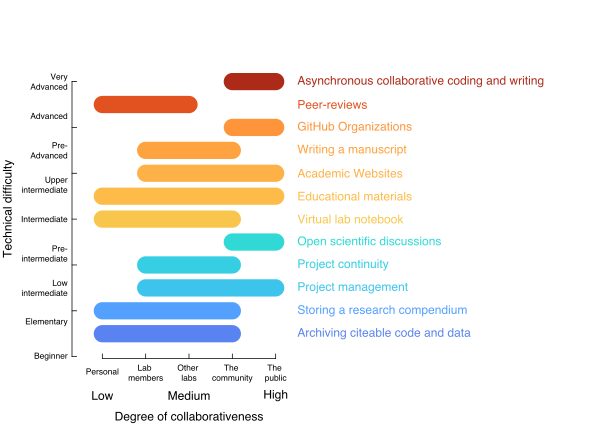
\includegraphics{images/scatterblob_1.png}
\caption{A summary of ways GitHub can be used showing technical difficulty and degree of collaboration for each. Activities higher on the vertical axis require usage knowledge of more GitHub features than activities lower on the axis. On the horizontal axis, each activity spans a region representing who is potentially involved with or benefits from each activity. For example, storing data and code mainly benefits individual researchers or members of a lab group while making data and code citable and reproducible benefit other labs and the larger community as well. Independently of a users knowledge level of GitHub features, there are ways to use GitHub that allow tapping unto one of the most salient benefits of the platform: facilitating and enhancing collaboration.}\label{fig:scatterblob}
}
\end{figure}

\hypertarget{tables}{%
\subsection{Tables}\label{tables}}

\begin{longtable}[]{@{}
  >{\raggedright\arraybackslash}p{(\columnwidth - 18\tabcolsep) * \real{0.0628}}
  >{\raggedright\arraybackslash}p{(\columnwidth - 18\tabcolsep) * \real{0.0529}}
  >{\raggedright\arraybackslash}p{(\columnwidth - 18\tabcolsep) * \real{0.0281}}
  >{\raggedright\arraybackslash}p{(\columnwidth - 18\tabcolsep) * \real{0.0281}}
  >{\raggedright\arraybackslash}p{(\columnwidth - 18\tabcolsep) * \real{0.0380}}
  >{\raggedright\arraybackslash}p{(\columnwidth - 18\tabcolsep) * \real{0.0529}}
  >{\raggedright\arraybackslash}p{(\columnwidth - 18\tabcolsep) * \real{0.1851}}
  >{\raggedright\arraybackslash}p{(\columnwidth - 18\tabcolsep) * \real{0.1669}}
  >{\raggedright\arraybackslash}p{(\columnwidth - 18\tabcolsep) * \real{0.2562}}
  >{\raggedright\arraybackslash}p{(\columnwidth - 18\tabcolsep) * \real{0.1289}}@{}}
\caption{a comparison of technologies commonly used for collaborating on research in Ecology and Evolutionary Biology. In the first column, we group platforms for collaboration into broad guilds. The second column lists the platform for collaboration. The remaining columns indicate whether the platform for collaboration includes certain features. \label{tbl:compare}}\tabularnewline
\toprule
\begin{minipage}[b]{\linewidth}\raggedright
Guild
\end{minipage} & \begin{minipage}[b]{\linewidth}\raggedright
Software
\end{minipage} & \begin{minipage}[b]{\linewidth}\raggedright
Vesion control
\end{minipage} & \begin{minipage}[b]{\linewidth}\raggedright
Backup (cloud)
\end{minipage} & \begin{minipage}[b]{\linewidth}\raggedright
Passive collaboration
\end{minipage} & \begin{minipage}[b]{\linewidth}\raggedright
Active real-time colalboration
\end{minipage} & \begin{minipage}[b]{\linewidth}\raggedright
Free \$
\end{minipage} & \begin{minipage}[b]{\linewidth}\raggedright
Permanent (DOI)
\end{minipage} & \begin{minipage}[b]{\linewidth}\raggedright
Storage limits
\end{minipage} & \begin{minipage}[b]{\linewidth}\raggedright
GitHub Integration
\end{minipage} \\
\midrule
\endfirsthead
\toprule
\begin{minipage}[b]{\linewidth}\raggedright
Guild
\end{minipage} & \begin{minipage}[b]{\linewidth}\raggedright
Software
\end{minipage} & \begin{minipage}[b]{\linewidth}\raggedright
Vesion control
\end{minipage} & \begin{minipage}[b]{\linewidth}\raggedright
Backup (cloud)
\end{minipage} & \begin{minipage}[b]{\linewidth}\raggedright
Passive collaboration
\end{minipage} & \begin{minipage}[b]{\linewidth}\raggedright
Active real-time colalboration
\end{minipage} & \begin{minipage}[b]{\linewidth}\raggedright
Free \$
\end{minipage} & \begin{minipage}[b]{\linewidth}\raggedright
Permanent (DOI)
\end{minipage} & \begin{minipage}[b]{\linewidth}\raggedright
Storage limits
\end{minipage} & \begin{minipage}[b]{\linewidth}\raggedright
GitHub Integration
\end{minipage} \\
\midrule
\endhead
Multi-tool & GitHub & yes & yes & yes & NA & Broadly limited free version. Advanced features are provided for free to students and education professionals. & A DOI can only be obtained when integrating to other services that can mint DOI (e.g.~Zenodo, OSF). & 100 MB per file, 500 MB per private repository (2 GB for paid accounts). 100 GB for public repositories. Larger files (up to 2 GB) can be attached to releases & NA \\
Multi-tool & OSF & yes & yes & yes & yes & yes & yes & 25 GB for private projects, up to 5GB per file, plus partner add-ons, 50GB for public projects & yes \\
Long-term (public) data repositories & PANGAEA & yes & yes & yes & NA & yes & yes & 10 GB free & NA \\
Long-term (public) data repositories & Zenodo & after published & after published & NA & NA & yes & yes & 50 GB per dataset & yes \\
Long-term (public) data repositories & Dryad & after published & after published & NA & NA & some journals cover cost & yes & 300 GB per publication & Can link to individual files (not entire reopository); not really integrated \\
Long-term (public) data repositories & Figshare & yes & yes & yes & NA & yes & yes & 20 GB free, up to 5 TB & yes \\
Temporary (personal) drive storage & Google Drive & yes & yes & yes & yes & limited free version \& paid & NA & 15 GB free, up to 100 GB with Google One & yes \\
Temporary (personal) drive storage & Box & limited & yes & ? & ? & NA & NA & Unlimited total size for subscription & yes \\
Temporary (personal) drive storage & DropBox & limited & yes & yes & yes & limited free version \& paid & NA & 2 GB free & yes \\
Temporary (personal) drive storage & One Drive and the Office Suite & yes & yes & yes & yes & limited free version \& paid & NA & 5 GB free, up to 1TB paid & yes \\
Collaborative code/text editors & Overleaf (online latex editor) & yes & yes & yes & NA & NA & NA & 1MB for individual .tex, 50 MB for individual files, unlimited project size & yes \\
Collaborative code/text editors & Jupyter Notebook & yes & ? & yes & with Colab & yes & NA & via Binder: no hard limit, but suggests no files \textgreater100 MB, can also store on GitHub or Google Colab & yes \\
Collaborative code/text editors & HackMD & yes & yes & yes & yes & yes & NA & 3 documents free, private invitee limits & yes \\
\bottomrule
\end{longtable}

\begin{longtable}[]{@{}
  >{\raggedright\arraybackslash}p{(\columnwidth - 14\tabcolsep) * \real{0.0493}}
  >{\raggedright\arraybackslash}p{(\columnwidth - 14\tabcolsep) * \real{0.1425}}
  >{\raggedright\arraybackslash}p{(\columnwidth - 14\tabcolsep) * \real{0.1041}}
  >{\raggedright\arraybackslash}p{(\columnwidth - 14\tabcolsep) * \real{0.1562}}
  >{\raggedright\arraybackslash}p{(\columnwidth - 14\tabcolsep) * \real{0.1096}}
  >{\raggedright\arraybackslash}p{(\columnwidth - 14\tabcolsep) * \real{0.1479}}
  >{\raggedright\arraybackslash}p{(\columnwidth - 14\tabcolsep) * \real{0.1370}}
  >{\raggedright\arraybackslash}p{(\columnwidth - 14\tabcolsep) * \real{0.1534}}@{}}
\caption{A non-exhaustive collection of ideas for how various GitHub
features could be utilized for a research project. Here we have
categorized contributors/collaborators into five roles. A Project
Manager owns the GitHub repository for a project, and leads the academic
project (e.g., lead author of a manuscript). A co-author contributes to
writing and other aspects of research, but may have limited or no
experience with programming, git, and/or GitHub. A code contributor
writes or edits analysis code for the project. A code reviewer could be
a project collaborator or a peer reviewer who reviews project code. They
are familiar with coding, but not necessarily with git or GitHub (but
they are willing to learn). Finally, community members could be other
researchers or non-researchers interested in reproducing results,
re-using code or data, or communicating with researchers involved in the
project. These roles are not mutually exclusive---a co-author could also
be e code contributor and code reviewer, for example. For definitions of
the GitHub features, see Box 1. \label{tbl:roles}}\tabularnewline
\toprule
\begin{minipage}[b]{\linewidth}\raggedright
Role
\end{minipage} & \begin{minipage}[b]{\linewidth}\raggedright
GitHub repository
\end{minipage} & \begin{minipage}[b]{\linewidth}\raggedright
README
\end{minipage} & \begin{minipage}[b]{\linewidth}\raggedright
Issue
\end{minipage} & \begin{minipage}[b]{\linewidth}\raggedright
Discussion
\end{minipage} & \begin{minipage}[b]{\linewidth}\raggedright
Pull Request
\end{minipage} & \begin{minipage}[b]{\linewidth}\raggedright
Fork
\end{minipage} & \begin{minipage}[b]{\linewidth}\raggedright
GitHub Pages
\end{minipage} \\
\midrule
\endfirsthead
\toprule
\begin{minipage}[b]{\linewidth}\raggedright
Role
\end{minipage} & \begin{minipage}[b]{\linewidth}\raggedright
GitHub repository
\end{minipage} & \begin{minipage}[b]{\linewidth}\raggedright
README
\end{minipage} & \begin{minipage}[b]{\linewidth}\raggedright
Issue
\end{minipage} & \begin{minipage}[b]{\linewidth}\raggedright
Discussion
\end{minipage} & \begin{minipage}[b]{\linewidth}\raggedright
Pull Request
\end{minipage} & \begin{minipage}[b]{\linewidth}\raggedright
Fork
\end{minipage} & \begin{minipage}[b]{\linewidth}\raggedright
GitHub Pages
\end{minipage} \\
\midrule
\endhead
Project manager & Set contributor permissions, share code of conduct & Project description, citation, DOIs & Assign tasks to collaborators & Discuss project directions and goals & Approve and incorporate edits to code and/or writing & & Share up-to-date reports, figures, or draft manuscript \\
Co-author & Edit Markdown text or add files & & Propose changes involving code (e.g.~analyses, figures) & Discuss proposed changes to manuscript & & & \\
Code contributor & & & Suggest code changes & & Contribute changes to code, initiate code review & & Contribute to project website \\
Code reviewer & Find all code related to a project & & Highlight specific lines of code and make suggestions & & Review or recommended changes in code & & \\
Community & & & Suggest additional features and report bugs & Ask questions about data and code & & Create a linked, editable copy of the repository & View project website \\
\bottomrule
\end{longtable}

\hypertarget{references}{%
\subsection{References}\label{references}}

\hypertarget{refs}{}
\begin{CSLReferences}{0}{0}
\leavevmode\vadjust pre{\hypertarget{ref-fJWFe93e}{}}%
\CSLLeftMargin{1. }
\CSLRightInline{Hannay, J. E. \emph{et al.} How do scientists develop and use scientific software? in \emph{2009 ICSE Workshop on Software Engineering for Computational Science and Engineering} (IEEE, 2009). doi:\href{https://doi.org/10.1109/secse.2009.5069155}{10.1109/secse.2009.5069155}.}

\leavevmode\vadjust pre{\hypertarget{ref-1Kqna6l2}{}}%
\CSLLeftMargin{2. }
\CSLRightInline{Perkel, J. M. \href{https://doi.org/10.1038/d41586-020-02462-7}{Challenge to scientists: does your ten-year-old code still run?} \emph{Nature} \textbf{584}, 656--658 (2020).}

\leavevmode\vadjust pre{\hypertarget{ref-10ghgV3S8}{}}%
\CSLLeftMargin{3. }
\CSLRightInline{Perkel, J. \href{https://doi.org/10.1038/538127a}{Democratic databases: science on GitHub}. \emph{Nature} \textbf{538}, 127--128 (2016).}

\leavevmode\vadjust pre{\hypertarget{ref-10SpoByIw}{}}%
\CSLLeftMargin{4. }
\CSLRightInline{Prabhu, P. \emph{et al.} A survey of the practice of computational science. in \emph{State of the Practice Reports on - SC '11} (ACM Press, 2011). doi:\href{https://doi.org/10.1145/2063348.2063374}{10.1145/2063348.2063374}.}

\leavevmode\vadjust pre{\hypertarget{ref-O6UbstGG}{}}%
\CSLLeftMargin{5. }
\CSLRightInline{Wilson, G. \emph{et al.} \href{https://doi.org/10.1371/journal.pbio.1001745}{Best Practices for Scientific Computing}. \emph{PLoS Biol} \textbf{12}, e1001745 (2014).}

\leavevmode\vadjust pre{\hypertarget{ref-nwCtHDCn}{}}%
\CSLLeftMargin{6. }
\CSLRightInline{Build software better, together. \emph{GitHub} \url{https://github.com}.}

\leavevmode\vadjust pre{\hypertarget{ref-RVetqmsg}{}}%
\CSLLeftMargin{7. }
\CSLRightInline{Bryan, J. \href{https://doi.org/10.1080/00031305.2017.1399928}{Excuse Me, Do You Have a Moment to Talk About Version Control?} \emph{The American Statistician} \textbf{72}, 20--27 (2018).}

\leavevmode\vadjust pre{\hypertarget{ref-4ny1onB0}{}}%
\CSLLeftMargin{8. }
\CSLRightInline{Ram, K. \href{https://doi.org/10.1186/1751-0473-8-7}{Git can facilitate greater reproducibility and increased transparency in science}. \emph{Source Code Biol Med} \textbf{8}, (2013).}

\leavevmode\vadjust pre{\hypertarget{ref-kEX5dgzK}{}}%
\CSLLeftMargin{9. }
\CSLRightInline{Perez-Riverol, Y. \emph{et al.} \href{https://doi.org/10.1371/journal.pcbi.1004947}{Ten Simple Rules for Taking Advantage of Git and GitHub}. \emph{PLoS Comput Biol} \textbf{12}, e1004947 (2016).}

\leavevmode\vadjust pre{\hypertarget{ref-13jOlVcpp}{}}%
\CSLLeftMargin{10. }
\CSLRightInline{Hester, J. B., the STAT 545 TAs, Jim. \emph{\href{https://happygitwithr.com/}{Let's Git started \textbar{} Happy Git and GitHub for the useR}}.}

\leavevmode\vadjust pre{\hypertarget{ref-u5aEVE4B}{}}%
\CSLLeftMargin{11. }
\CSLRightInline{Coding Club: A Positive Peer-Learning Community. \url{https://ourcodingclub.github.io/}.}

\leavevmode\vadjust pre{\hypertarget{ref-3DKwn1sY}{}}%
\CSLLeftMargin{12. }
\CSLRightInline{Lowndes, J. S. S. \emph{et al.} \href{https://doi.org/10.1038/s41559-017-0160}{Our path to better science in less time using open data science tools}. \emph{Nat Ecol Evol} \textbf{1}, (2017).}

\leavevmode\vadjust pre{\hypertarget{ref-139b0pSGc}{}}%
\CSLLeftMargin{13. }
\CSLRightInline{Leibzon, W. Social network of software development at GitHub. in \emph{2016 IEEE/ACM International Conference on Advances in Social Networks Analysis and Mining (ASONAM)} (IEEE, 2016). doi:\href{https://doi.org/10.1109/asonam.2016.7752419}{10.1109/asonam.2016.7752419}.}

\leavevmode\vadjust pre{\hypertarget{ref-ydrk01SR}{}}%
\CSLLeftMargin{14. }
\CSLRightInline{Briney, K., Coates, H. \& Goben, A. \href{https://doi.org/10.3897/rio.6.e56508}{Foundational Practices of Research Data Management}. \emph{RIO} \textbf{6}, (2020).}

\leavevmode\vadjust pre{\hypertarget{ref-13QX8XU3J}{}}%
\CSLLeftMargin{15. }
\CSLRightInline{Alston, J. M. \& Rick, J. A. \href{https://doi.org/10.1002/bes2.1801}{A Beginner's Guide to Conducting Reproducible Research}. \emph{Bull. Ecol. Soc. Am.} \textbf{102}, (2021).}

\leavevmode\vadjust pre{\hypertarget{ref-pq2Tv1BC}{}}%
\CSLLeftMargin{16. }
\CSLRightInline{Gomes, D. G. E. \emph{et al.} Why don't we share data and code? Perceived barriers and benefits to public archiving practices. (2022) doi:\href{https://doi.org/10.31222/osf.io/gaj43}{10.31222/osf.io/gaj43}.}

\leavevmode\vadjust pre{\hypertarget{ref-MwwMapRG}{}}%
\CSLLeftMargin{17. }
\CSLRightInline{Marwick, B., Boettiger, C. \& Mullen, L. \href{https://doi.org/10.1080/00031305.2017.1375986}{Packaging Data Analytical Work Reproducibly Using R (and Friends)}. \emph{The American Statistician} \textbf{72}, 80--88 (2018).}

\leavevmode\vadjust pre{\hypertarget{ref-1Co6ZZjF1}{}}%
\CSLLeftMargin{18. }
\CSLRightInline{About large files on GitHub. \emph{GitHub Docs} \url{https://ghdocs-prod.azurewebsites.net/en/repositories/working-with-files/managing-large-files/about-large-files-on-github}.}

\leavevmode\vadjust pre{\hypertarget{ref-11GtZ7icJ}{}}%
\CSLLeftMargin{19. }
\CSLRightInline{Git Large File Storage. \emph{Git Large File Storage} \url{https://git-lfs.github.com/}.}

\leavevmode\vadjust pre{\hypertarget{ref-wwHxTOtm}{}}%
\CSLLeftMargin{20. }
\CSLRightInline{Kanza, S. \emph{et al.} \href{https://doi.org/10.1186/s13321-017-0221-3}{Electronic lab notebooks: can they replace paper?} \emph{J Cheminform} \textbf{9}, (2017).}

\leavevmode\vadjust pre{\hypertarget{ref-10V7x4H4l}{}}%
\CSLLeftMargin{21. }
\CSLRightInline{Schnell, S. \href{https://doi.org/10.1371/journal.pcbi.1004385}{Ten Simple Rules for a Computational Biologist's Laboratory Notebook}. \emph{PLoS Comput Biol} \textbf{11}, e1004385 (2015).}

\leavevmode\vadjust pre{\hypertarget{ref-RhBKe0MG}{}}%
\CSLLeftMargin{22. }
\CSLRightInline{About projects (beta). \emph{GitHub Docs} \url{https://ghdocs-prod.azurewebsites.net/en/issues/trying-out-the-new-projects-experience/about-projects}.}

\leavevmode\vadjust pre{\hypertarget{ref-1GRWGlDWy}{}}%
\CSLLeftMargin{23. }
\CSLRightInline{Slack. GitHub for Slack. \emph{Slack Help Center} \url{https://slack.com/help/articles/232289568-GitHub-for-Slack}.}

\leavevmode\vadjust pre{\hypertarget{ref-QqMezOMg}{}}%
\CSLLeftMargin{24. }
\CSLRightInline{Xie, Y., Allaire, J. J. \& Grolemund, G. \emph{R Markdown: the definitive guide}. (CRC Press, Taylor and Francis Group, 2019).}

\leavevmode\vadjust pre{\hypertarget{ref-MDQfMwCW}{}}%
\CSLLeftMargin{25. }
\CSLRightInline{Quickstart for GitHub Pages. \emph{GitHub Docs} \url{https://ghdocs-prod.azurewebsites.net/en/pages/quickstart}.}

\leavevmode\vadjust pre{\hypertarget{ref-dqrFjoSb}{}}%
\CSLLeftMargin{26. }
\CSLRightInline{Trujillo, G. \& Tanner, K. D. \href{https://doi.org/10.1187/cbe.13-12-0241}{Considering the Role of Affect in Learning: Monitoring Students' Self-Efficacy, Sense of Belonging, and Science Identity}. \emph{LSE} \textbf{13}, 6--15 (2014).}

\leavevmode\vadjust pre{\hypertarget{ref-HiIPSSHV}{}}%
\CSLLeftMargin{27. }
\CSLRightInline{Smaglik, P. \href{https://doi.org/10.1038/nj7142-347a}{Creating better lab websites gives potential collaborators and recruiters a clearer window into your world.} \emph{Nature} \textbf{447}, 347--347 (2007).}

\leavevmode\vadjust pre{\hypertarget{ref-MXxgZJ45}{}}%
\CSLLeftMargin{28. }
\CSLRightInline{Dawson, C. \emph{Building tools with GitHub: customize your workflow}. (O'Reilly, 2016).}

\leavevmode\vadjust pre{\hypertarget{ref-PLmDFZrm}{}}%
\CSLLeftMargin{29. }
\CSLRightInline{Tenopir, C. \emph{et al.} \href{https://doi.org/10.1371/journal.pone.0229003}{Data sharing, management, use, and reuse: Practices and perceptions of scientists worldwide}. \emph{PLoS ONE} \textbf{15}, e0229003 (2020).}

\leavevmode\vadjust pre{\hypertarget{ref-1Hcf13Q0k}{}}%
\CSLLeftMargin{30. }
\CSLRightInline{Nugroho, R. P., Zuiderwijk, A., Janssen, M. \& de Jong, M. \href{https://doi.org/10.1108/tg-03-2014-0008}{A comparison of national open data policies: lessons learned}. \emph{Transforming Government: People, Process and Policy} \textbf{9}, 286--308 (2015).}

\leavevmode\vadjust pre{\hypertarget{ref-1Ch6LSHef}{}}%
\CSLLeftMargin{31. }
\CSLRightInline{Wicherts, J. M., Bakker, M. \& Molenaar, D. \href{https://doi.org/10.1371/journal.pone.0026828}{Willingness to Share Research Data Is Related to the Strength of the Evidence and the Quality of Reporting of Statistical Results}. \emph{PLoS ONE} \textbf{6}, e26828 (2011).}

\leavevmode\vadjust pre{\hypertarget{ref-SLq38RVv}{}}%
\CSLLeftMargin{32. }
\CSLRightInline{Figueiredo, A. S. \href{https://doi.org/10.3389/fpubh.2017.00327}{Data Sharing: Convert Challenges into Opportunities}. \emph{Front. Public Health} \textbf{5}, (2017).}

\leavevmode\vadjust pre{\hypertarget{ref-1CzUZwyU2}{}}%
\CSLLeftMargin{33. }
\CSLRightInline{Tenopir, C. \emph{et al.} \href{https://doi.org/10.1371/journal.pone.0134826}{Changes in Data Sharing and Data Reuse Practices and Perceptions among Scientists Worldwide}. \emph{PLoS ONE} \textbf{10}, e0134826 (2015).}

\leavevmode\vadjust pre{\hypertarget{ref-666HppfO}{}}%
\CSLLeftMargin{34. }
\CSLRightInline{Pronk, T. E., Wiersma, P. H., van Weerden, A. \& Schieving, F. \href{https://doi.org/10.7717/peerj.1242}{A game theoretic analysis of research data sharing}. \emph{PeerJ} \textbf{3}, e1242 (2015).}

\leavevmode\vadjust pre{\hypertarget{ref-1CcAUn3Lu}{}}%
\CSLLeftMargin{35. }
\CSLRightInline{Piwowar, H. A., Day, R. S. \& Fridsma, D. B. \href{https://doi.org/10.1371/journal.pone.0000308}{Sharing Detailed Research Data Is Associated with Increased Citation Rate}. \emph{PLoS ONE} \textbf{2}, e308 (2007).}

\leavevmode\vadjust pre{\hypertarget{ref-4LaijDIZ}{}}%
\CSLLeftMargin{36. }
\CSLRightInline{\href{https://doi.org/10.1038/ncb3506}{On data availability, reproducibility and reuse}. \emph{Nat Cell Biol} \textbf{19}, 259--259 (2017).}

\leavevmode\vadjust pre{\hypertarget{ref-uBJwnPbq}{}}%
\CSLLeftMargin{37. }
\CSLRightInline{Mislan, K. A. S., Heer, J. M. \& White, E. P. \href{https://doi.org/10.1016/j.tree.2015.11.006}{Elevating The Status of Code in Ecology}. \emph{Trends in Ecology \&amp; Evolution} \textbf{31}, 4--7 (2016).}

\leavevmode\vadjust pre{\hypertarget{ref-1HZdsK5Kn}{}}%
\CSLLeftMargin{38. }
\CSLRightInline{Baker, M. \href{https://doi.org/10.1038/533452a}{1,500 scientists lift the lid on reproducibility}. \emph{Nature} \textbf{533}, 452--454 (2016).}

\leavevmode\vadjust pre{\hypertarget{ref-1Du6fzB8g}{}}%
\CSLLeftMargin{39. }
\CSLRightInline{Crystal‐Ornelas, R. \emph{et al.} \href{https://doi.org/10.1029/2021ea001797}{A Guide to Using GitHub for Developing and Versioning Data Standards and Reporting Formats}. \emph{Earth Space Sci} \textbf{8}, (2021).}

\leavevmode\vadjust pre{\hypertarget{ref-iIEKCTLU}{}}%
\CSLLeftMargin{40. }
\CSLRightInline{Hampton, S. E. \emph{et al.} \href{https://doi.org/10.1890/es14-00402.1}{The Tao of open science for ecology}. \emph{Ecosphere} \textbf{6}, art120 (2015).}

\leavevmode\vadjust pre{\hypertarget{ref-TOsASkn5}{}}%
\CSLLeftMargin{41. }
\CSLRightInline{Adding a license to a repository. \emph{GitHub Docs} \url{https://ghdocs-prod.azurewebsites.net/en/communities/setting-up-your-project-for-healthy-contributions/adding-a-license-to-a-repository}.}

\leavevmode\vadjust pre{\hypertarget{ref-1BJcvyTmV}{}}%
\CSLLeftMargin{42. }
\CSLRightInline{Vale, G., Schmid, A., Santos, A. R., de Almeida, E. S. \& Apel, S. \href{https://doi.org/10.1007/s10664-019-09774-x}{On the relation between Github communication activity and merge conflicts}. \emph{Empir Software Eng} \textbf{25}, 402--433 (2019).}

\leavevmode\vadjust pre{\hypertarget{ref-K7nbP1Ty}{}}%
\CSLLeftMargin{43. }
\CSLRightInline{Crystal-Ornelas, R. \emph{et al.} \emph{Not just for programmers: How GitHub can accelerate collaborative and reproducible research in ecology and evolution}. \url{https://SORTEE-Github-Hackathon.github.io/manuscript/} (2022).}

\leavevmode\vadjust pre{\hypertarget{ref-hm9PaCLD}{}}%
\CSLLeftMargin{44. }
\CSLRightInline{Song, X., Goldstein, S. C. \& Sakr, M. Using Peer Code Review as an Educational Tool. in \emph{Proceedings of the 2020 ACM Conference on Innovation and Technology in Computer Science Education} (ACM, 2020). doi:\href{https://doi.org/10.1145/3341525.3387370}{10.1145/3341525.3387370}.}

\leavevmode\vadjust pre{\hypertarget{ref-YuJbg3zO}{}}%
\CSLLeftMargin{45. }
\CSLRightInline{Himmelstein, D. S. \emph{et al.} \href{https://doi.org/10.1371/journal.pcbi.1007128}{Open collaborative writing with Manubot}. \emph{PLoS Comput Biol} \textbf{15}, e1007128 (2019).}

\leavevmode\vadjust pre{\hypertarget{ref-Xsdcv6q}{}}%
\CSLLeftMargin{46. }
\CSLRightInline{Boettiger, C., Lang, D. T. \& Wainwright, P. C. \href{https://doi.org/10.1111/j.1095-8649.2012.03464.x}{rfishbase: exploring, manipulating and visualizing FishBase data from R}. \emph{Journal of Fish Biology} \textbf{81}, 2030--2039 (2012).}

\leavevmode\vadjust pre{\hypertarget{ref-FVBWKkZu}{}}%
\CSLLeftMargin{47. }
\CSLRightInline{Chamberlain, S. A. \& Szöcs, E. \href{https://doi.org/10.12688/f1000research.2-191.v2}{taxize: taxonomic search and retrieval in R}. \emph{F1000Res} \textbf{2}, 191 (2013).}

\leavevmode\vadjust pre{\hypertarget{ref-NOgBWVAr}{}}%
\CSLLeftMargin{48. }
\CSLRightInline{Culina, A., van den Berg, I., Evans, S. \& Sánchez-Tójar, A. \href{https://doi.org/10.1371/journal.pbio.3000763}{Low availability of code in ecology: A~call for urgent action}. \emph{PLoS Biol} \textbf{18}, e3000763 (2020).}

\leavevmode\vadjust pre{\hypertarget{ref-18PTmKJkq}{}}%
\CSLLeftMargin{49. }
\CSLRightInline{January 18, P. L. B. K. \& Pm, 2022. 2:51. \#PruittData and the Ethics of Data in Science. \emph{Ecology for the Masses} \url{https://ecologyforthemasses.com/2020/02/04/pruittdata-and-the-ethics-of-data-in-science/} (2020).}

\leavevmode\vadjust pre{\hypertarget{ref-D4C4k4ak}{}}%
\CSLLeftMargin{50. }
\CSLRightInline{Fehr, J., Himpe, C., Rave, S. \& Saak, J. \href{https://doi.org/10.5334/jors.307}{Sustainable Research Software Hand-Over}. \emph{JORS} \textbf{9}, 5 (2021).}

\leavevmode\vadjust pre{\hypertarget{ref-19kmNxiHc}{}}%
\CSLLeftMargin{51. }
\CSLRightInline{Vines, Timothy~H. \emph{et al.} \href{https://doi.org/10.1016/j.cub.2013.11.014}{The Availability of Research Data Declines Rapidly with Article Age}. \emph{Current Biology} \textbf{24}, 94--97 (2014).}

\leavevmode\vadjust pre{\hypertarget{ref-s91uGRZ2}{}}%
\CSLLeftMargin{52. }
\CSLRightInline{About code owners. \emph{GitHub Docs} \url{https://ghdocs-prod.azurewebsites.net/en/repositories/managing-your-repositorys-settings-and-features/customizing-your-repository/about-code-owners}.}

\leavevmode\vadjust pre{\hypertarget{ref-UsTxAq4f}{}}%
\CSLLeftMargin{53. }
\CSLRightInline{Anbaroğlu, B. \href{https://doi.org/10.1111/tgis.12810}{A collaborative GIS programming course using GitHub Classroom}. \emph{Transactions in GIS} \textbf{25}, 3132--3158 (2021).}

\leavevmode\vadjust pre{\hypertarget{ref-lx49NGto}{}}%
\CSLLeftMargin{54. }
\CSLRightInline{Connect GitHub to a Project - OSF Support. \url{https://help.osf.io/article/211-connect-github-to-a-project}.}

\leavevmode\vadjust pre{\hypertarget{ref-pjy75gHr}{}}%
\CSLLeftMargin{55. }
\CSLRightInline{Madicken Munk \emph{et al.} swcarpentry/git-novice: Software Carpentry: Version Control with Git, June 2019. at \url{https://doi.org/10.5281/zenodo.3264950} (2019).}

\leavevmode\vadjust pre{\hypertarget{ref-ZvrOcg9w}{}}%
\CSLLeftMargin{56. }
\CSLRightInline{Hester, J. B., the STAT 545 TAs, Jim. \emph{\href{https://happygitwithr.com/}{Let's Git started \textbar{} Happy Git and GitHub for the useR}}.}

\leavevmode\vadjust pre{\hypertarget{ref-6CMMeSeD}{}}%
\CSLLeftMargin{57. }
\CSLRightInline{Bryan, J. \& TAs, T. S. 545. \emph{\href{https://stat545.com/}{STAT 545}}.}

\end{CSLReferences}
